\newpage

\section{Hauptteil} \label{Methodik}
In diesem Kapitel wird die Methodik der Arbeit beschrieben. Zunächst wird das CRISP-DM Modell vorgestellt, welches als Grundlage für die Durchführung der Arbeit dient. Anschließend wird erläutert, wie dieses Modell in der Arbeit angewendet wird, um die Forschungsfrage zu beantworten.

ToDo: evt. noch eine Begründung warum CRISP-DM gewählt wurde

\subsection{Überblick CRISP-DM Modell} \label{ueberblickcrispdm}
Das CRISP-DM Modell (Cross-Industry Standard Process for Data Mining) ist ein bewährtes und strukturiertes Modell für Data Mining Projekte. 
CRISP-DM wurde 1996 durch ein Konsortium bestehend aus Daimler-Benz, SPSS, NCR und der niederländischen Versicherungsgesellschaft OHRA konzipiert und 2000 in der Version 1.0 veröffentlicht. (vgl. Zitat: "CRISP-DM 1.0: A Standard Process Model for Data Mining", Shearer, C., 2000).
Das Modell hat sich als de facto Standard in der Data Mining Community etabliert und wird laut verschiedenen Umfragen von 2002, 2004, 2007 und 2014 als führende Methodik von Data Mining Experten verwendet. (vgl. Zitat Data Science Central, 2016).

Das Modell unterteilt den Prozess des Data Mining in sechs verschiedene Phasen.

\begin{figure}[ht]
    \centering
    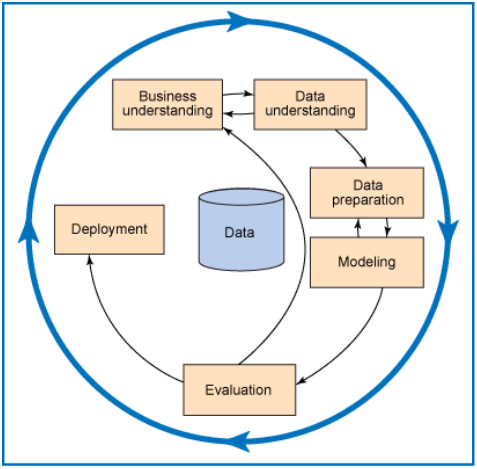
\includegraphics[width=0.7\textwidth]{figures/crispdm.png}
    \caption{Die 6 Phasen des CRISP-DM Modells}
    \label{fig:crispdm}
\end{figure}

Das besondere an diesem Vorgehen ist, dass es an die teils nicht-lineare struktur von KI oder Deep Learning Projekten (vgl. Zitat Data Science Central, 2026) angepasst ist. Auch ein iteratives Vorgehen, welches in solchen Projekten angewendet wird, kann mit dem CRISP-DM Modell abgebildet werden wie auch in der Abbildung \ref{fig:crispdm} zu sehen ist. Das ist wichtig da die Schritte in der Praxis oft nicht linear abgearbeitet werden können und es wichtig ist die Flexibilität zu haben, vorherige Schritte zu wiederholen um deren Resultate zu verbessern oder anzupassen.

Um ein tieferes und besseres Verständnis für die sechs Phasen des CRISP-DM Modells in der Theorie zu bekommen, werden diese im Folgenden kurz beschrieben. In dem darauf folgenden Unterkapitel wird erläutert, wie diese Phasen in der Arbeit angewendet werden, um die Forschungsfrage zu beantworten.

\textbf{Business Understanding:} bildet die Grundlage des Projekts und fokussiert sich auf das Verständnis der Projektziele und die Anforderungen aus geschäftlicher Perspektive.

\textbf{Data Understanding:} eine erste Datensammlung wird durchgeführt, um ein initiales Verständnis für die Daten zu bekommen. Im Fokus steht hier die Identifikation relevanter Datenquellen sowie die Sammlung von Daten und die erste Analyse der Daten, um deren Qualität und Struktur zu bewerten.

\textbf{Data Preparation:} aufbereitung der Daten und Vorbereitung für die Modellierung. Die Phase umfasst die Bereinigung und Transformation der Daten in ein geeignetes Format und die Auswahl relevanter Features für die Modellierung.

\textbf{Modeling:} Beim Modeling werden verschiedene Modelle entwickelt und getestet, um die analytischen Ziele zu erreichen. Dies umfasst die Auswahl geeigneter Modellierungstechniken, die Entwicklung von Modellen und die Bewertung der Modelle hinsichtlich ihrer Leistung.

\textbf{Evaluation:} hier werden die entwickelten Modelle bewertet und überprüft hinsichtlich ihrer Erfüllung der gestellten Anforderungen. Die Phase umfasst die Überprüfung der Modellleistung sowie die Validierung der Modelle und die Entscheidung, ob das Modell in der Praxis eingesetzt werden kann.

\textbf{Deployment:} In der finalen Phase wird das entwickelte Modell in der Praxis verwendet. Hier wird das Modell implementiert, im Betrieb überwacht und bei Bedarf angepasst.

\subsection{Anwendung des Modells in dieser Arbeit} \label{anwendungdesmodellsinderarbeit}
\textbf{Business Understanding}

\textbf{Data Understanding}

\textbf{Data Preparation}

\textbf{Modeling}

\textbf{Evaluation}

\textbf{Deployment}





Business Understanding

    Zieldefinition: Bewertung, ob der Deutschlandatlas als Datenquelle geeignet ist, um Immobilienkaufpreise in Deutschland zu ermitteln und vorherzusagen.

    Ableitung konkreter Analyseziele: Entwicklung eines Vorhersagemodells für Immobilienpreise auf Basis der im Deutschlandatlas verfügbaren Indikatoren.

    Identifikation relevanter Stakeholder (z.B. Immobilienunternehmen, Investoren, Politik).

Data Understanding

    Sichtung und Analyse der im Deutschlandatlas bereitgestellten Daten (z.B. sozioökonomische Indikatoren, regionale Kennzahlen).

    Überprüfung der Datenverfügbarkeit bezüglich Immobilienkaufpreisen und potenziell relevanter Einflussfaktoren.

    Erste Exploration: Identifizieren von Korrelationen zwischen Atlasdaten und Immobilienpreisen.

    Erkennen von Datenlücken oder potenziellen Verzerrungen.

Data Preparation

    Auswahl relevanter Variablen aus dem Deutschlandatlas (z.B. Einkommen, Arbeitslosenquote, Infrastruktur).

    Ergänzung durch externe Quellen, falls direkte Immobilienpreisdaten fehlen.

    Datenbereinigung: Umgang mit fehlenden Werten, Ausreißern und Inkonsistenzen.

    Transformation und Aggregation der Daten auf die gewünschte regionale Ebene (z.B. Landkreise, Städte).

Modeling

    Auswahl geeigneter Modellierungsmethoden (z.B. lineare Regression, Random Forest).

    Training der Modelle mit den aufbereiteten Daten.

    Feature Engineering: Auswahl und Kombination von Variablen, die Immobilienpreise beeinflussen könnten.

    Durchführung von Modellvalidierungen (z.B. Kreuzvalidierung).

Evaluation

    Bewertung der Modellgüte anhand geeigneter Metriken (z.B. RMSE, R²).

    Überprüfung, ob die Modelle auf Basis der Deutschlandatlas-Daten verlässliche Vorhersagen ermöglichen.

    Analyse der wichtigsten Einflussfaktoren im Modell.

    Reflexion, inwieweit die Forschungsfrage beantwortet werden kann.

Deployment

    Präsentation der Ergebnisse in verständlicher Form (z.B. Visualisierungen, Karten).

    Diskussion der Implikationen für Praxis und Forschung.

    Empfehlungen für die Nutzung des Deutschlandatlas in der Immobilienmarktanalyse.

    Hinweise auf Limitationen und mögliche Weiterentwicklungen.

